\documentclass[a4paper,11pt]{article}

\usepackage{graphicx}
\graphicspath{{figures/}}
\usepackage{amsmath}
\usepackage{amssymb}
\usepackage{booktabs}
\usepackage{hyperref}
\usepackage{geometry}
\usepackage{caption}
\usepackage{siunitx}
\usepackage{titlesec}
\usepackage{float}
\geometry{top=0.5in, right=0.45in, left=0.45in, bottom=0.5in}

\captionsetup[table]{labelfont=small}
\captionsetup[figure]{labelfont=small}

\title{Take-Home, Advanced Microeconomics (20296)\\[0.2em]\large Problem 1: Overworked Americans: Q1, Q4, Q5, Q7}
\author{Alessandro Caggia (3178115), Stefano De Bianchi (3154360), Eduard Hartel (3378615), Francesco Mastidoro (3323853)}
\date{May 2026}

\titlespacing*{\section}{0pt}{8pt}{6pt}
\titlespacing*{\subsection}{0pt}{6pt}{2pt}
\titlespacing*{\paragraph}{0pt}{4pt}{0.6em}
\captionsetup{aboveskip=3pt, belowskip=-6pt}
\linespread{1}
\emergencystretch=2em
\widowpenalty=10000
\clubpenalty=10000

\begin{document}

\makeatletter
\renewcommand{\maketitle}{
    \begingroup
    \vspace{-1.5cm}
    \centering
    {\LARGE \bfseries \@title \par}
    \vskip 1em
    {\large \@author \par}
    \vskip 1em
    {\normalsize \@date \par}
    \vskip 1em
    \endgroup
}
\makeatother
\maketitle

% =========================================================================
\section{Q1 -- The hours gap and its noisy relation to tax wedges\protect\footnote{\emph{Methodological note.} Q4 and Q5 each show that their respective channel can absorb the residual the Prescott mechanism leaves unexplained; Q7 is where these channels are confronted with the US--EU mapping and the welfare verdict is rendered. This comparative structure is deliberate: the prompt's substantive question asks for conditions, not for the maximum reach of any single channel, so we go broad across the institutional menu rather than deep in one --- with formal Lagrangians, regularity conditions, and comparative statics relegated to Appendices~\ref{app:q4} and~\ref{app:q5}. The payoff is a result no single-channel treatment could produce: a fairness-belief gap between US and EU recovered from observed bargaining institutions (\S 5.3, Reading B).}}
% =========================================================================

\begingroup\small\itshape\noindent\textbf{Question 1.} Document the EU--US (and intra-EU) hours-worked gap in recent years.\endgroup\footnote{\emph{Definitions.} For the working-age (15--64) population: hours per employed worker $HE$ (the intensive object the labour-supply model speaks to), employment rate $e\!\equiv\!E/N$, hours per adult $H/N\!\equiv\!HE\cdot e$. The Bick--Br\"uggemann--Fuchs-Sch\"undeln (2019) decomposition $\Delta\log(H/N)\!=\!\Delta\log HE\!+\!\Delta\log e$ assigns roughly half of the EU--US gap to each margin; we focus on $HE$. The extensive margin is shut down throughout (cross-country $e$ differences are substantial: US $71\%$ vs IT $59\%$ in 2019), but the prompt asks about hours, so $HE$ is the relevant object.}

\subsection{The fact}
\begin{figure}[H]
\centering

\includegraphics[width=\textwidth]{figure_panel.pdf}
\caption{\small\textbf{Three-panel evidence.} (a) Hours per worker, \% deviation from US, 1970--2024 (OECD). (b) Effective labour wedge $\tau_h$, \% deviation from US, 1970--2007. (c) OECD labour-tax wedge vs hours per worker, 2023 cross-section ($n\!=\!19$); OLS line and $\pm 1\sigma_\text{resid}$ band.}
\label{fig:gapPanel}
\end{figure}

Three readings of Figure~\ref{fig:gapPanel}. \textbf{(i)} Hours fell in every focus country relative to the US since 1970 (DE/NL $\approx -25$ to $-30\%$; IT/ES $\approx -10$ to $-15\%$). \textbf{(ii)} The labour-wedge cross-country pattern has no clean structure: Italy's relative wedge drifts up, the UK's narrows, France stays roughly flat, no obvious mirroring of the panel-(a) hours pattern. \textbf{(iii)} The 2023 cross-section is signed correctly but noisy: OLS slope $-9.9$\,hrs/pp, $R^2\!=\!0.16$, residual SD $\approx\!158$ hours, one third of the entire DE--US gap. Italy ($\tau\!=\!45.1\%$) and Greece ($36.7\%$) work \emph{more} than France ($46.8\%$); the four highest-$\tau$ countries (BE, DE, AT, FR) span $\approx\!200$ hours within a 6\,pp wedge band. Panel (c) thus motivates two questions: the true slope of the tax--hours relation (OLS-biased by $\tau$ endogeneity), and the wide residual scatter around it ($\approx\!158$ hours SD), into which Q4 and Q5 develop two institutional channels, an hours cap and union bargaining, as endogenous confounders.\footnote{Other candidates we do not model: leisure complementarity / cultural attitudes to work (Alesina, Glaeser \& Sacerdote 2005), and home-production substitution.}

% =========================================================================
\section{Common framework for Q4 and Q5}
% =========================================================================

\subsection{Primitives}
We adopt a quadratic-disutility worker, linear consumption, and a linear-quadratic firm-profit function, the simplest closed-form specification that admits both worker- and firm-preferred hours and sign-determinate welfare conditions:
\[
V_w(h)=(1-\tau)wh-\tfrac{\alpha}{2}h^2,\;\; h^*=\frac{(1-\tau)w}{\alpha}; \qquad
V_f(h)=Ah-\tfrac{\beta}{2}h^2-wh,\;\; h^{\mathrm{firm}}=\frac{A-w}{\beta}.
\]
Joint surplus is $W(h)\!\equiv\!V_w(h)+V_f(h)\!=\!Ah-\tau wh-\tfrac{\alpha+\beta}{2}h^2$. The wage transfer cancels between worker and firm; only the tax wedge $\tau wh$ survives. $W$ is concave with maximum
\[
h^{\mathrm{soc}}(\tau,\alpha,A,\beta,w)  = \frac{A-\tau w}{\alpha+\beta}.
\]
The setup is shared by Q4 (regulation) and Q5 (unions). Wages are partial-equilibrium throughout.

\subsection{Baseline calibration and the firm-power ordering}
$A\!=\!2$, $w\!=\!1$, $\alpha\!=\!\beta\!=\!2$, $\tau\!=\!0.4$, $V_w^{0}\!=\!0.05$ gives $h^*\!=\!0.30$, $h^{\mathrm{soc}}\!=\!0.40$, $h^{\mathrm{firm}}\!=\!0.50$. \textbf{Justification of the parameter choices.} (i) $\tau\!=\!0.4$ is the population-weighted midpoint between US ($0.35$) and EU ($0.56$) labour-tax wedges (OECD \emph{Taxing Wages 2023}, Q1 panel (c)). (ii) The hours scale anchors $h^*\!=\!0.30$ to BLS-OECD hours-per-worker over awake-time at the US point ($\sim\!2{,}000$ work hours / $\sim\!6{,}500$ awake hours $\approx\!0.31$, in line with standard macro-labour calibrations). (iii) $\alpha\!=\!\beta$ is a symmetry assumption that makes the welfare-improving band of \eqref{eq:capwelf} collapse to the textbook expression $(h^*,h^{\mathrm{firm}})$, but \textbf{only the ordering $h^*\!<\!h^{\mathrm{soc}}\!<\!h^{\mathrm{firm}}$ is load-bearing} for what follows; the qualitative results are invariant in $\alpha,\beta$ separately, provided $A\!>\!w$, $\tau\!\in\!(0,1)$, and the sufficient condition $\alpha(A-w)>\beta(1-\tau)w$ holds (algebraically equivalent to the ordering; verified at calibration: $2\!=\!\alpha(A-w)>\beta(1-\tau)w\!=\!1.2$). (iv) $A\!=\!2,\,w\!=\!1$ are normalisations: the level of $A$ is identified only relative to $w$, and our results depend on the ratio $A/w$, not the absolute scale. (v) $V_w^{0}\!=\!0.05$ is the worker outside option used to pin the IR-binding wage. It is jointly determined with $w\!=\!1$: at the firm-power baseline IR binds, so $V_w(h^{\mathrm{firm}};w\!=\!1)\!=\!(1-\tau)w h^{\mathrm{firm}}-\tfrac{\alpha}{2}(h^{\mathrm{firm}})^{2}\!=\!0.05$ recovers $V_w^{0}$. The discriminant condition $A_v^{2}\!>\!4B_v V_w^{0}$ for a real larger root of \eqref{eq:rtm-quad} is verified in Appendix~\ref{app:q5}.

The ordering says that, when the firm has all the bargaining power, it overshoots the social optimum. We refer to this as the \emph{firm-power baseline} (the firm sets hours on its labour-demand curve at the wage that makes the worker indifferent between working and her outside option). With identical $\tau$ and identical preferences, the model predicts no US--EU hours gap under firm power \emph{or} under union bargaining: the gap must come from a country-specific institutional asymmetry, which Q4 (cap) and Q5 (union strength) supply.

% =========================================================================
\section{Q4 -- Hours regulation: the optimality condition for a cap}
% =========================================================================


\subsection{Modelling choice}
A cap $\bar h$ is a quantity instrument that takes the firm's labour-demand response as given. \emph{What the trade-off captures.} Workers value leisure (low $h^*$); firms value output (high $h^{\mathrm{firm}}$); a binding cap forces hours from $h^{\mathrm{firm}}$ toward $\bar h$. Whether the redistribution is welfare-improving depends on whether $\bar h$ lands inside or outside the welfare-improving band defined by joint-surplus concavity: too tight a cap overshoots and destroys joint surplus. \emph{What this buys.} A closed-form welfare condition that depends only on the gap $h^{\mathrm{firm}}\!-\!h^{\mathrm{soc}}$. \emph{What it costs.} (a) Extensive margin shut down (Q1 footnote): no firm response on number of bodies hired. (b) Wages held at the firm-power IR-binding level (no adjustment of $w$ to absorb the cap). (c) Representative-worker setup (homogeneous preferences). The closest sufficient-statistics analogue is the minimum-wage literature, but its welfare logic runs through extensive-margin rationing whereas a binding hours cap rations \emph{intensive}-margin only.

\subsection{Setup: firm-power baseline}
At $w^*\!=\!1$ pinning the worker's IR at $V_w^0$, the firm picks $h^{\mathrm{firm}}\!=\!(A-w^*)/\beta\!=\!0.50$. Hours sit \emph{above} $h^{\mathrm{soc}}\!=\!0.40$, so the cap has something to correct. With cap $\bar h$ the constrained equilibrium is $h^{\mathrm{eq}}(\bar h)\!=\!\min\{\bar h,\,h^{\mathrm{firm}}\}$.

\subsection{Worker, firm, and joint surplus under a cap}
The three surpluses, evaluated at $h^{\mathrm{eq}}(\bar h)$ relative to the no-cap baseline, are quadratic in $\bar h$ around the respective bliss points:
\begin{center}\footnotesize
\begin{tabular}{lll}
\toprule
Surplus & Closed form (for $\bar h<h^{\mathrm{firm}}$) & Sign \\
\midrule
$\Delta V_w(\bar h)=V_w(\bar h)-V_w(h^{\mathrm{firm}})$ & $(\bar h-h^{\mathrm{firm}})\bigl[(1-\tau)w-\tfrac{\alpha}{2}(\bar h+h^{\mathrm{firm}})\bigr]$ & $>0$ iff $\bar h\!\in\!(2h^{*}-h^{\mathrm{firm}},\,h^{\mathrm{firm}})$\\
$\Delta V_f(\bar h)=V_f(\bar h)-V_f(h^{\mathrm{firm}})$ & $-\tfrac{\beta}{2}(h^{\mathrm{firm}}-\bar h)^{2}$ & $<0$ for any $\bar h<h^{\mathrm{firm}}$\\
$\Delta W(\bar h)=\Delta V_w+\Delta V_f$ & $-\tfrac{\alpha+\beta}{2}\bigl[(h^{\mathrm{soc}}-\bar h)^{2}-(h^{\mathrm{soc}}-h^{\mathrm{firm}})^{2}\bigr]$ & $>0$ iff $\bar h\!\in\!(2h^{\mathrm{soc}}-h^{\mathrm{firm}},\,h^{\mathrm{firm}})$\\
\bottomrule
\end{tabular}
\end{center}

\subsection{Optimality condition (the Q4 result)}
Full Lagrangian/FOC derivation of \eqref{eq:capwelf} is in Appendix~\ref{app:q4}.

\textbf{Claim.} Joint surplus $W(h)$ is strictly concave and quadratic with peak at $h^{\mathrm{soc}}$, so $W(\bar h)$ is symmetric in $\bar h$ around $h^{\mathrm{soc}}$. The function $\Delta W(\bar h)$ equals zero at $\bar h\!=\!h^{\mathrm{firm}}$ (no cap) and at the mirror point $2h^{\mathrm{soc}}\!-\!h^{\mathrm{firm}}$, and is positive between them:
\begin{equation}
\Delta W(\bar h)   \begin{cases} =0 & \text{if } \bar h\geq h^{\mathrm{firm}}\\ >0 & \text{iff } \bar h\in\bigl(2h^{\mathrm{soc}}-h^{\mathrm{firm}},\,h^{\mathrm{firm}}\bigr)\\ <0 & \text{if } \bar h<2h^{\mathrm{soc}}-h^{\mathrm{firm}} \end{cases}
\label{eq:capwelf}
\end{equation}
provided $h^{\mathrm{firm}}>h^{\mathrm{soc}}$ (which holds at our baseline, $0.50\!>\!0.40$). The peak gain at $\bar h\!=\!h^{\mathrm{soc}}$ is $\tfrac{1}{2}(\alpha+\beta)(h^{\mathrm{firm}}-h^{\mathrm{soc}})^{2}\!=\!0.020$ at calibration. At $\alpha\!=\!\beta$ the band collapses to $\bar h\!\in\!(h^*,h^{\mathrm{firm}})\!=\!(0.30,0.50)$.

\textbf{Reading.} A cap that pulls $h$ \emph{toward} the joint-surplus optimum is unambiguously welfare-improving (the green band of Figure~\ref{fig:simcap}c). Two thresholds matter as the cap tightens past $h^{\mathrm{soc}}$. Joint surplus turns negative once $\bar h\!<\!2h^{\mathrm{soc}}-h^{\mathrm{firm}}\!=\!h^{*}\!=\!0.30$ (firm losses begin to dominate worker gains). The worker individually keeps benefiting until the cap hits her bliss $h^{*}\!=\!0.30$; she only becomes worse off than no-cap once the cap tightens further to $\bar h\!<\!2h^{*}-h^{\mathrm{firm}}\!=\!0.10$, well below the joint-surplus threshold (Appendix~\ref{app:q4}).

\begin{figure}[H]
\centering

\includegraphics[width=\textwidth]{sim_cap.pdf}
\caption{\small\textbf{Hours-cap simulation.} \textbf{(a)} Primitives $V_w, V_f, W$ over $h$ with bliss points marked; \textbf{(b)} surpluses along $h^{\mathrm{eq}}(\bar h)\!=\!\min\{\bar h,h^{\mathrm{firm}}\}$; \textbf{(c)} $\Delta W(\bar h)$ vs no-cap baseline, green band is the welfare-improving region of \eqref{eq:capwelf}, red is overshoot. Maximum gain $\Delta W\!=\!0.020$ at $\bar h\!=\!h^{\mathrm{soc}}\!=\!0.40$.}
\label{fig:simcap}
\end{figure}

\textbf{Empirical anchor.} The 35-hour Aubry reform (France 1998--2000) documented by Estev\~ao--S\'a (2008) found $\approx\!10\!-\!13\%$ hours cut and near-zero employment effect, consistent with a binding cap at $\bar h/h^{\mathrm{firm}}\!\approx\!0.875$ inside the welfare-improving band of \eqref{eq:capwelf}.\footnote{The near-zero employment effect is consistent with our model only because we have shut down the extensive margin (see the Q1 footnote): if a binding cap reduces hours per worker, firms may substitute workers for hours, an effect the representative-agent setup rules out by construction. Sectoral composition (a large public sector with multi-year collective contracts) is also outside the model.}

% =========================================================================
\section{Q5 -- A single union as welfare-restorer in a two-sector economy}
% =========================================================================


\subsection{Modelling choice}
\emph{What the trade-off captures.} The Walrasian benchmark rewards productivity through wages, so a sectoral shock is absorbed by reallocating hours; the union changes the channel of absorption (wages take more, hours take less) and, under downward wage rigidity, makes that channel asymmetric across positive and negative shocks. \emph{What this buys.} A single bargain primitive ($\eta$) delivers a continuous comparative static between the firm-power baseline ($\eta\!=\!0$) and the worker-power limit ($\eta\!\to\!1$), nesting the Q4 distortion and the Walrasian benchmark as endpoints. \emph{What it costs.} (a) A single encompassing union, following Calmfors--Driffill (1988): encompassing (national/centralised) unions internalise their macroeconomic effect, so their objective aligns with worker surplus rather than with subgroup rent extraction, letting us match the European centralised-bargaining institutional reality. (b) Right-to-manage instead of efficient bargaining, the standard tractability convention for unionised wage-setting. (c) Informal labour and the public sector are outside the model.\footnote{An alternative model would have the union charge a share $s$ of worker income to finance itself; the union's revenue then scales with worker income, so its incentive maps directly onto worker surplus and the alignment result below is unchanged.}

\subsection{Two-sector economy: competitive benchmark}
Two sectors $j\!\in\!\{\textsc{g},\textsc{b}\}$ (good, bad) with productivities $A_{\textsc{g}}\!>\!A_{\textsc{b}}$, drawn from a mean-preserving sectoral shock around a symmetric pre-shock benchmark $A_{\rm pre}\!=\!2$ (we set $A_{\textsc{g}}\!=\!2.2$, $A_{\textsc{b}}\!=\!1.8$, a $\pm 10\%$ shock chosen as a conservative magnitude for developed-world cross-sectoral TFP dispersion (the developing-country literature documents substantially wider dispersion, so this magnitude sits below that range)). Within each sector a representative worker--firm pair has the quadratic primitives of \S 3.

\textbf{Competitive (Walrasian) benchmark.} With perfect labour mobility across sectors, sector wages clear at the marginal value product: the firm's labour demand is $h_j^d(w)\!=\!(A_j-w)/\beta$, and the worker's IR pins $w_j^{\rm FM}$ such that hours equal $h^{\mathrm{firm}}_j(w_j^{\rm FM})$. The headline competitive comparative static is:
\[
\frac{\partial h_j^{\rm FM}}{\partial A_j} > 0,\qquad \frac{\partial w_j^{\rm FM}}{\partial A_j} > 0.
\]
\emph{Hours follow productivity}: positive shocks raise hours and wages in the good sector; negative shocks lower them in the bad sector. Cross-sectoral allocation is efficient given the shock.

\subsection{Two-sector economy: unionised version}
A single union covers both sectors. Per sector, union and firm right-to-manage Nash-bargain over $w_j$ with worker weight $\eta\!\in\!(0,1)$:
\begin{equation}
w_j(\eta;A_j)=\arg\max_w\, \bigl[V_w(w,h_j^d(w))-V_w^{\,0}\bigr]^{\eta}\; V_f(w,h_j^d(w);A_j)^{1-\eta},\qquad h_j^d(w)=(A_j-w)/\beta.
\label{eq:rtm-bargain}
\end{equation}
The first-order condition reduces to a quadratic in $x_j\!\equiv\!A_j\!-\!w_j$ (Appendix~\ref{app:q5}) with limits $h_j(0)\!=\!h^{\mathrm{firm}}_j$ and $h_j(1)\!<\!h^{*}(w_j(1))$; $\partial w_j/\partial\eta>0$, $\partial h_j/\partial\eta<0$ throughout.

\textbf{Welfare-restorer.} Under the firm-power baseline $h^{\mathrm{firm}}_j\!>\!h^{\mathrm{soc}}_j\!>\!h_j^{*}$, so as $\eta$ rises the union pulls hours \emph{toward} the social optimum: joint surplus rises while $h_j(\eta)\!\in\!(h^{\mathrm{soc}}_j,h^{\mathrm{firm}}_j)$ and falls thereafter, the overshoot logic of Q4. Worker surplus is monotone in $\eta$, so any planner with positive worker weight strictly prefers $\eta\!>\!0$.

\textbf{US vs.\ EU calibration.} OECD ICTWSS coverage maps US ($\sim\!12\%$) to $\eta^{\,US}\!\approx\!0.15$ and population-weighted EU coverage ($\sim\!60$--$70\%$ across DE/FR/IT/SE under \emph{erga omnes}) to $\eta^{\,EU}\!\approx\!0.5$. At these calibrated values we get $h^{\,US}\!\approx\!0.46$ at $\eta^{\,US}\!=\!0.15$ and EU mean hours $\tfrac{1}{2}(h_{\textsc{g}}\!+\!h_{\textsc{b}})\!\approx\!0.38$ at $\eta^{\,EU}\!=\!0.5$ (sectoral $h_{\textsc{g}}\!\approx\!0.42$, $h_{\textsc{b}}\!\approx\!0.33$), an EU--US gap of order $\approx\!0.08$ ($\approx\!19\%$ in logs), the right order of magnitude to absorb a substantial fraction of the gap documented in Q1.

\subsection{Sectoral shocks: union pass-through and asymmetry}
Substituting $A_{\textsc{g}}, A_{\textsc{b}}$ into \eqref{eq:rtm-bargain} at $\eta\!=\!0.5$ (Figure~\ref{fig:simshocks}): $w_{\textsc{g}}^{\,U}\!=\!1.354,\,h_{\textsc{g}}^{\,U}\!=\!0.423$ and $w_{\textsc{b}}^{\,U}\!=\!1.132,\,h_{\textsc{b}}^{\,U}\!=\!0.334$. The good sector splits the productivity gain into wages ($\Delta w/w\!\approx\!+25\%$) and reduced hours ($\Delta h/h\!\approx\!-24\%$); joint surplus falls only $\approx\!5\%$ ($W_g^{\rm FM}\!=\!0.363\to W_g^{U}\!=\!0.344$), with the bulk of the redistribution being a wage-rent transfer rather than a deadweight loss.

\textbf{Asymmetry under downward wage rigidity.} If unions refuse to renegotiate wages downward, the bad-sector wage is stuck at $w_{\rm pre}\!=\!1.242$ and hours collapse to $(A_{\textsc{b}}-w_{\rm pre})/\beta\!=\!0.279$ ($36\%$ below free market; firm profit $60\%$ below). Headline: \textbf{good shocks pass through diluted (absorbed in wage rents); bad shocks pass through amplified (rigidity forces hours to absorb the entire shock)}.

\begin{figure}[H]
\centering

\includegraphics[width=\textwidth]{sim_shocks.pdf}
\caption{\small\textbf{Asymmetric pass-through under three regimes.} \textbf{(a)} Labour-demand shifts and equilibria: rigid bad-sector equilibrium sits on the new demand at the stuck pre-shock wage. \textbf{(b)} Hours response: good-sector hours rise under all regimes; bad-sector rigid is $36\%$ below free market. \textbf{(c)} Firm profit: good-sector profit rises under all regimes; bad-sector rigid is $60\%$ below free market.}
\label{fig:simshocks}
\end{figure}

\subsection{Data to test the hypotheses}
Three falsifiable predictions: (a) hours decrease in union bargaining strength conditional on productivity; (b) the US--EU gap rises with the coverage gap; (c) bad-sector shocks generate larger hours responses in unionised economies. Required data: sectoral hours panels (OECD STAN, EU KLEMS), coverage by sector (ICTWSS), collective-agreement wage indices. Identification of the rigidity asymmetry exploits the post-2000 manufacturing decline in DE and IT, where sectoral hours and employment fell sharply but real wages did not.

% =========================================================================
\section{Q7 -- Welfare comparison: a revealed-preference reading}
% =========================================================================


\subsection{Modelling choice}
The Q4 cap and the Q5 union, in our specification, are both quantity instruments that pull hours from $h^{\mathrm{firm}}$ toward $h^{\mathrm{soc}}$.\footnote{We focus on hours throughout. The wage channel is implicit: the union's effect on $h$ operates through a bargained wage premium, and the Saez--Stantcheva $\lambda$ assigns welfare value to the firm-to-worker transfer that this premium effects. We do not separately analyse cross-country wage differences, which the prompt does not ask about and our partial-equilibrium calibration cannot speak to.} Whether a given configuration is welfare-enhancing depends on \emph{whose} welfare we are summing. The natural representation of the cross-country welfare disagreement is the Saez--Stantcheva (2016) generalised welfare weight: the planner attaches premium $\lambda\!\in\![0,1]$ to a worker dollar over a firm-owner dollar,
\[
W^{\lambda}(\eta) = (1+\lambda)\,V_w(\eta) + (1-\lambda)\,V_f(\eta).
\]
$\lambda\!=\!0$ is equal-weight utilitarianism, $\lambda\!=\!1$ is Rawlsian. Following Alesina--Angeletos (2005), $\lambda$ is a country-specific primitive: it captures fairness beliefs (whether income inequality is seen as deserved or as luck), which can differ across countries even at common preferences and technology. We compare the two systems through the lens of this single parameter.

\subsection{Welfare-optimum bargaining weight: closed form}
Maximising $W^{\lambda}(\eta)$ along the bargained path of \eqref{eq:rtm-bargain} gives the welfare-optimum reduced-form variable $x^{*}\!\equiv\!A-w^{*}\!=\!\beta h^{*}$:
\[
x^{*}(\lambda)\;=\;\frac{0.3\,A\,(1+\lambda)}{0.6+1.6\,\lambda}\qquad\text{(at baseline)}.
\]
Substituting $x^{*}(\lambda)$ into the Nash-bargain quadratic recovers the \emph{welfare-optimum bargaining weight}:
\[
\eta^{*}(\lambda) = \frac{1.2\,x^{*}-1.1\,(x^{*})^{2}-0.1}{0.6\,x^{*}-0.1}.
\]
$\eta^{*}$ is monotonically increasing in $\lambda$, with $\eta^{*}(0)\!=\!0$ (firm-power optimal under equal weights) and $\eta^{*}(1)\!=\!1$ (full union under Rawlsian).

\subsection{Confronting data: observed unionisation in US and EU}
We map the Nash-bargain weight $\eta$ to OECD bargaining-coverage data: $\hat\eta^{\,US}\!\approx\!0.15$ (coverage $\sim\!12\%$), $\hat\eta^{\,EU}\!\approx\!0.50$ (coverage $\sim\!60\%$ population-weighted across DE/FR/IT/SE).\footnote{The mapping is a coarse linear proxy: it overstates Nordic high-density regimes and understates French \emph{erga omnes} extension regimes, where coverage is high but bargaining power is weak.} These two observations admit two competing readings.

\paragraph{Reading A, common $\lambda$.} If both countries share the Heathcote--Storesletten--Violante (2017) progressivity index $\tau_p\!\approx\!0.18$, which under log preferences maps to $\lambda\!\approx\!0.30$, the welfare-optimum is $\eta^{*}(0.30)\!=\!0.58$, so the US ($\hat\eta\!=\!0.15$) is heavily under-unionised and the EU ($\hat\eta\!=\!0.50$) only mildly. The implied losses $W^{0.30}(\eta^{*})-W^{0.30}(\hat\eta)$ are $0.022$ for the US and $0.001$ for the EU, the US leaves $\sim\!8\%$ of joint surplus on the table. We flag this reading but do not endorse it (see Reading B).

\paragraph{Reading B, country-specific $\lambda$ (preferred).} Inverting $\eta^{*}(\lambda)$ on observed coverage:
\[
\hat\eta^{\,US}\!=\!0.15\;\Longrightarrow\;\lambda^{\,US,\rm rev}\!\approx\!0.05,\qquad
\hat\eta^{\,EU}\!=\!0.50\;\Longrightarrow\;\lambda^{\,EU,\rm rev}\!\approx\!0.24.
\]
Each country's institutions are at-optimum given its own fairness primitive ($\Delta\lambda\!\approx\!0.19$); the union-channel hours drag is small in the US ($h^{\mathrm{firm}}\!\to\!0.45$, $-9\%$) and larger in the EU ($h^{\mathrm{firm}}\!\to\!0.38$, $-24\%$). \textbf{Verdict.} Neither country is welfare-better in absolute terms, each implements its own optimum, and the EU--US hours gap reflects a fairness-belief gap rather than institutional misalignment, supplying the missing variable in Q1 panel (c). The data prefer this reading over A (Figure~\ref{fig:simq7etalambda}): Reading A would put all countries on the horizontal line $\eta\!=\!\eta^{*}(0.30)$, which the observed range (US 0.15, FR 0.98, SE 0.88, DE 0.52) clearly violates.\footnote{The cap channel (Q4) is orthogonal at our calibration: the union alone pulls $h$ below any sensible cap, so Q4 is a counterfactual backstop, not an active driver. Outside the labour-market block, dominant US--EU welfare differences run through non-labour channels (life expectancy, consumption levels); our verdict is sign-determinate but quantitatively second-order.}

\begin{figure}[H]
\centering
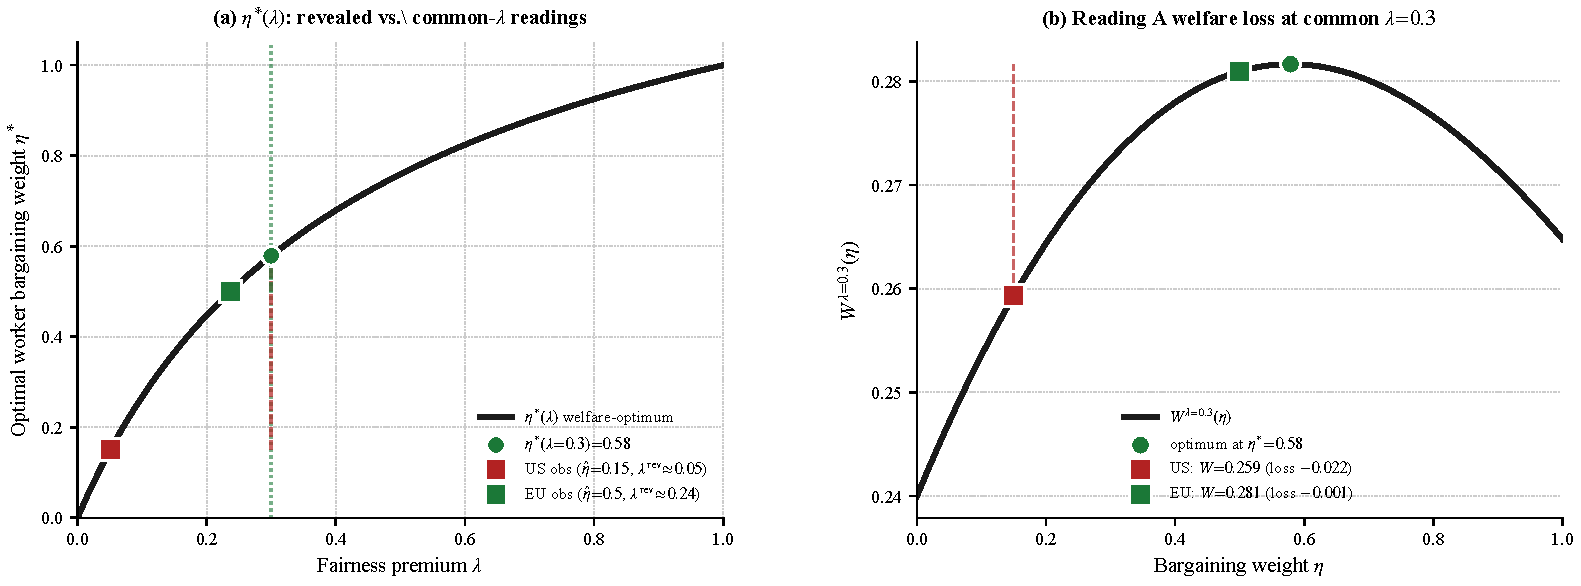
\includegraphics[width=0.78\textwidth]{sim_q7_eta_lambda.pdf}
\caption{\small \textbf{Q7 revealed-preference diagnostic.} \textbf{(a)} The $\eta^{*}(\lambda)$ welfare-optimum locus (black). Observed US and EU points sit on the locus at their revealed-preference $\lambda^{\rm rev}$ (Reading B). Vertical dashed segments show the deviation under common $\lambda\!=\!0.30$ (Reading A): both countries below the optimum, US far more so. \textbf{(b)} $W^{\lambda\!=\!0.30}(\eta)$: peak at $\eta^{*}\!=\!0.58$. US loss $-0.022$ (under-unionised by 0.43); EU loss $-0.001$ (essentially at-optimum).}
\label{fig:simq7etalambda}
\end{figure}

% =========================================================================
\section*{References}
\begingroup
\setlength{\parindent}{-1.2em}\setlength{\leftskip}{1.2em}
\footnotesize

Alesina, A., \& Angeletos, G.-M.\ (2005). Fairness and Redistribution. \emph{AER} 95(4), 960--980 [\textbf{Q7 country-specific $\lambda$}].

Alesina, A., Glaeser, E., \& Sacerdote, B.\ (2005). Work and Leisure in the United States and Europe: Why So Different? \emph{NBER Macroeconomics Annual} 20, 1--64 [\textbf{Q1 cultural-attitudes alternative}].

Bick, A., Br\"uggemann, B., \& Fuchs-Sch\"undeln, N.\ (2019). Hours Worked in Europe and the US: New Data, New Answers. \emph{Scandinavian Journal of Economics} 121(4), 1381--1416 [\textbf{Q1 H/N decomposition}].

Calmfors, L., \& Driffill, J.\ (1988). Bargaining Structure, Corporatism and Macroeconomic Performance. \emph{Economic Policy} 3(6), 13--61 [\textbf{Q5 encompassing-union foundation}].

Estev\~ao, M., \& S\'a, F.\ (2008). The 35-Hour Workweek in France: Straightjacket or Welfare Improvement? \emph{Economic Policy} 23(55), 418--463 [\textbf{Q4 Aubry empirical anchor}].

Heathcote, J., Storesletten, K., \& Violante, G.\ L.\ (2017). Optimal Tax Progressivity: An Analytical Framework. \emph{QJE} 132(4), 1693--1754 [\textbf{Q7 $\lambda\!=\!0.30$ calibration anchor}].

Saez, E., \& Stantcheva, S.\ (2016). Generalized Social Marginal Welfare Weights for Optimal Tax Theory. \emph{AER} 106(1), 24--45 [\textbf{Q7 $\lambda$-weighted welfare}].

\medskip
\noindent\emph{Replication scripts in \texttt{research/}: \texttt{build\_figure\_panel.py} (Q1 figure); \texttt{sim\_models\_v2.py} (Q5 RTM and sectoral shocks); \texttt{sim\_mechanisms.py} (Q4 cap simulation).}
\endgroup

\section{Formal derivation of the Q4 cap results}\label{app:q4}
% =========================================================================

\noindent\emph{Unabridged \S A.1, \S A.2 in companion \href{https://github.com/AlessandroCaggia30/overworked-americans-takehome/blob/main/appendix_full.pdf}{\texttt{appendix\_full.pdf}}.}

\subsection{Primitives, FOCs, and the three bliss points}
From $V_w(h)=(1-\tau)wh-\tfrac{\alpha}{2}h^{2}$ and $V_f(h)=Ah-\tfrac{\beta}{2}h^{2}-wh$:
\[
h^{*}=\frac{(1-\tau)w}{\alpha},\quad h^{\mathrm{firm}}=\frac{A-w}{\beta},\quad h^{\mathrm{soc}}=\arg\max\bigl[V_w+V_f\bigr]=\frac{A-\tau w}{\alpha+\beta}.
\]
At baseline: $(h^{*},h^{\mathrm{soc}},h^{\mathrm{firm}})=(0.30,\,0.40,\,0.50)$.

\subsection{Firm's constrained programme under a cap}
The firm picks $h$ to maximise $V_f$ s.t.\ $h\le\bar h$, with $w$ pinned by IR $V_w(h)=V_w^{0}$.\footnote{Without IR the firm pushes $w$ arbitrarily low for unbounded rents; IR pins $w$ at the level matching the worker's outside option.} KKT on the cap-only sub-problem yields
\[
h^{\mathrm{eq}}(\bar h)=\min\{\bar h,\,h^{\mathrm{firm}}\},\qquad \mu=\max\{0,\,A-w-\beta\bar h\}.
\]

\subsection{Quadratic identities for the three surpluses}
Any concave quadratic with bliss $h^{\dagger}$ and curvature $-\kappa$ satisfies $g(h)-g(h^{\dagger})=-\tfrac{\kappa}{2}(h-h^{\dagger})^{2}$. Applied to $V_f$ (bliss $h^{\mathrm{firm}}$, curvature $\beta$) and $W$ (bliss $h^{\mathrm{soc}}$, curvature $\alpha+\beta$):
\begin{align}
\Delta V_f(\bar h) &= -\tfrac{\beta}{2}(h^{\mathrm{firm}}-\bar h)^{2}, \label{eq:dVf}\\
\Delta W(\bar h) &= -\tfrac{\alpha+\beta}{2}\bigl[(h^{\mathrm{soc}}-\bar h)^{2}-(h^{\mathrm{soc}}-h^{\mathrm{firm}})^{2}\bigr]. \label{eq:dW}
\end{align}
$\Delta V_w$ is not centred at the worker's bliss; direct expansion and the factorisation $\bar h^{2}-(h^{\mathrm{firm}})^{2}=(\bar h-h^{\mathrm{firm}})(\bar h+h^{\mathrm{firm}})$ give
\begin{equation}
\Delta V_w(\bar h)=(\bar h-h^{\mathrm{firm}})\bigl[(1-\tau)w-\tfrac{\alpha}{2}(\bar h+h^{\mathrm{firm}})\bigr]. \label{eq:dVw}
\end{equation}

\subsection{Welfare-improving band: derivation of \texorpdfstring{\eqref{eq:capwelf}}{Eq.\ (1)}}
For $\bar h<h^{\mathrm{firm}}$, \eqref{eq:dW} gives $\Delta W>0\iff |h^{\mathrm{soc}}-\bar h|<h^{\mathrm{firm}}-h^{\mathrm{soc}}\iff \bar h\in(2h^{\mathrm{soc}}-h^{\mathrm{firm}},\,h^{\mathrm{firm}})$, the welfare-improving band of \eqref{eq:capwelf}. Peak at $\bar h=h^{\mathrm{soc}}$:
\[
\Delta W(h^{\mathrm{soc}})=\tfrac{\alpha+\beta}{2}(h^{\mathrm{firm}}-h^{\mathrm{soc}})^{2}=0.020.
\]
At $\alpha=\beta$, $2h^{\mathrm{soc}}-h^{\mathrm{firm}}=(1-\tau)w/\beta=h^{*}$, so the band simplifies to $(h^{*},h^{\mathrm{firm}})=(0.30,0.50)$.

\subsection{Worker-surplus band and the two thresholds}\label{app:q4-worker-band}
For $\bar h<h^{\mathrm{firm}}$ the leading factor in \eqref{eq:dVw} is negative, so $\Delta V_w>0$ iff the bracket is also negative, i.e.\ $\bar h>2h^{*}-h^{\mathrm{firm}}$. Combined with cap binding:
\begin{equation}
\Delta V_w(\bar h)>0\iff \bar h\in\bigl(2h^{*}-h^{\mathrm{firm}},\,h^{\mathrm{firm}}\bigr),
\label{eq:cap-worker-band}
\end{equation}
with peak at the worker's bliss: $\Delta V_w(h^{*})=\tfrac{\alpha}{2}(h^{\mathrm{firm}}-h^{*})^{2}=0.04$.

\textbf{The two thresholds.} The joint threshold $2h^{\mathrm{soc}}-h^{\mathrm{firm}}$ weakly exceeds the worker threshold $2h^{*}-h^{\mathrm{firm}}$ since $h^{\mathrm{soc}}\!\ge\!h^{*}$ (equality only at $\tau\!=\!0$). At baseline they are $(0.30,\,0.10)$: for $\bar h\!\in\!(0.10,0.30)$ the cap is welfare-reducing on aggregate (firm losses dominate) but the individual worker still gains.

% =========================================================================
\section{Formal derivation of the Q5 RTM bargain}\label{app:q5}
% =========================================================================

\noindent\emph{Unabridged \S B.1--\S B.7 in companion \href{https://github.com/AlessandroCaggia30/overworked-americans-takehome/blob/main/appendix_full.pdf}{\texttt{appendix\_full.pdf}}.}

\subsection{Composite payoffs and bargained equilibrium}
With $h^d_j(w)=(A_j-w)/\beta$ and $x_j\equiv A_j-w$, the composite primitives are
\[
V_w(x_j)=A_v x_j-B_v x_j^{2},\qquad V_f(x_j)=\frac{x_j^{2}}{2\beta},
\]
where $A_v\!\equiv\!(1-\tau)A_j/\beta$ and $B_v\!\equiv\!(1-\tau)/\beta+\alpha/(2\beta^{2})$. The interior FOC of the asymmetric Nash product $[V_w-V_w^{0}]^{\eta}V_f^{1-\eta}$ reduces to the quadratic
\begin{equation}
2B_v x_j^{2}-A_v(2-\eta)\,x_j+2(1-\eta)\,V_w^{0}=0,
\label{eq:rtm-quad}
\end{equation}
whose larger root $x_j^{\star}(\eta)$ delivers the bargained $w_j=A_j-x_j^{\star}$, $h_j=x_j^{\star}/\beta$. At baseline this reads $1.1\,x^{2}-0.3A_j(2-\eta)x+0.1(1-\eta)=0$: $(A,\eta)=(2,0)\Rightarrow x^{\star}=1$ ($w=1,\,h=0.5$); $(A_g,\eta)=(2.2,0.5)\Rightarrow x^{\star}\!\approx\!0.846$ ($w\!\approx\!1.354,\,h\!\approx\!0.423$, Figure~\ref{fig:simshocks}).

\subsection{Boundary conditions}
\emph{(i)} $\eta\!=\!0$: \eqref{eq:rtm-quad} becomes $V_w(x_j)\!=\!V_w^{0}$ (IR binds), so $h_j\!=\!h^{\mathrm{firm}}_j$.
\emph{(ii)} $\eta\!\to\!1$: $2B_v x^{2}-A_v x=0$ with non-trivial root $x_j^{\star}(1)\!=\!A_v/(2B_v)$, giving $h_j(1)\!=\!(1-\tau)A_j/[2\beta(1-\tau)+\alpha]$. The SOC bracket $4B_v x-A_v(2-\eta)$ at this point equals $A_v\!>\!0$, so the limit is a maximum, not a corner.

\subsection{Walrasian benchmark and comparative statics in $A_j$}\label{app:q5-walras}
\textbf{Maintained regularity.} \emph{(R1)} $A_v^{2}\!>\!4B_vV_w^{0}$ (real distinct roots); \emph{(R2)} $x_j^{\mathrm{FM}}(A_j)^{2}>2\beta^{2}V_w^{0}/\alpha$.\footnote{At calibration: (R1) $0.36>0.11$. (R2) $x_j^{\mathrm{FM}}\!=\!1$ vs.\ threshold $0.2$; on $A_j\!\in\![1.8,2.2]$ the worst case $x_b\!=\!0.878$ gives $x^{2}\!=\!0.771>0.2$.}

The free-market larger root is $x_j^{\mathrm{FM}}(A_j)=[A_v+\sqrt{A_v^{2}-4B_v V_w^{0}}]/(2B_v)$. Implicit differentiation of $V_w(x_j;A_j)\!=\!V_w^{0}$ gives
\[
\frac{\partial x_j^{\mathrm{FM}}}{\partial A_j}=\frac{(1-\tau)\,x_j^{\mathrm{FM}}}{\beta(2B_v x_j^{\mathrm{FM}}-A_v)}>0
\]
(denominator positive: larger root past parabola vertex). Substituting the IR identity $A_v x\!=\!B_v x^{2}+V_w^{0}$ rewrites this as $(1-\tau)x^{2}/[\beta(B_v x^{2}-V_w^{0})]<1$ under (R2). So
\[
\partial h_j^{\mathrm{FM}}/\partial A_j>0,\qquad \partial w_j^{\mathrm{FM}}/\partial A_j>0
\]
``Hours and wages follow productivity'' under perfect labour mobility.

\subsection{Comparative statics in $\eta$ and the welfare-restorer claim}
Implicit differentiation of \eqref{eq:rtm-quad}:
\[
\bigl[4B_v x_j-A_v(2-\eta)\bigr]\frac{dx_j}{d\eta}=-A_v x_j+2V_w^{0}.
\]
The bracket on the LHS equals $\sqrt{D(\eta)}$, where $D(\eta)\!\equiv\!A_v^{2}(2-\eta)^{2}-16B_v(1-\eta)V_w^{0}$ is the discriminant of \eqref{eq:rtm-quad}; under (R1), $D>0$ on $[0,1]$.\footnote{$D(\eta)$ is a quadratic in $\eta$ with positive leading $A_v^{2}$ and minimum $16B_vV_w^{0}(A_v^{2}-4B_vV_w^{0})/A_v^{2}>0$ under (R1); at calibration the vertex sits at $\eta_v\!=\!1.39\!\notin\![0,1]$.} The RHS is strictly negative since $A_v x_j^{\star}\ge A_v^{2}/(2B_v)>2V_w^{0}$ by (R1). So
\[
\frac{dx_j}{d\eta}<0,\qquad \frac{dw_j}{d\eta}>0,\qquad \frac{dh_j}{d\eta}<0.
\]

\textbf{Welfare-restorer.} $W$ is concave with peak at $h^{\mathrm{soc}}_j\!\in\!(h^{*}_j,h^{\mathrm{firm}}_j)$. Since $h_j(\eta)$ is continuous, strictly decreasing, with $h_j(0)\!=\!h^{\mathrm{firm}}_j$, IVT delivers a unique $\hat\eta_j\!\in\!(0,1)$ with $h_j(\hat\eta_j)\!=\!h^{\mathrm{soc}}_j$. Combined with the quadratic identity \eqref{eq:dW},
\[
W\bigl(h_j(\eta)\bigr)-W\bigl(h^{\mathrm{firm}}_j\bigr)=-\tfrac{\alpha+\beta}{2}\Bigl[(h^{\mathrm{soc}}_j-h_j(\eta))^{2}-(h^{\mathrm{soc}}_j-h^{\mathrm{firm}}_j)^{2}\Bigr]
\]
is increasing on $[0,\hat\eta_j]$ (toward the social optimum) and decreasing thereafter (overshoot). Worker surplus is monotone in $\eta$: $V_w(x)$ is concave with peak at $\hat x\!=\!A_v/(2B_v)\!=\!x_j^{\star}(1)$, and $x_j^{\star}(\eta)\!\in\!(\hat x,x_j^{\star}(0)]$ on $[0,1)$ where $V_w'<0$, so $dV_w/d\eta\!=\!V_w'\cdot dx_j^{\star}/d\eta>0$ (product of two negatives). Any planner with positive worker weight $\lambda$ in the Q7 weighting $W^{\lambda}=(1+\lambda)V_w+(1-\lambda)V_f$ therefore strictly prefers $\eta\!>\!0$.

\end{document}
